\documentclass[aspectratio=169,usenames,dvipsnames]{beamer}
\beamertemplatenavigationsymbolsempty
% \documentclass{beamer}

% UNCOMMENT FOR HANDOUTS
% \usepackage{pgfpages}
% \pgfpagesuselayout{2 on 1}[landscape,letterpaper,border shrink=5mm]
% \setbeameroption{show notes}

\mode<presentation>
\usetheme{Boadilla}
\usecolortheme{spruce}
\usepackage{../../LizStyle,ulem}
\usepackage{color}
\usepackage[color,matrix,arrow]{xy}
% \input xy
% \xyoption{all}
\usepackage{tikz}
\usepackage{tikz-cd}
\tikzset{commutative diagrams/diagrams={ampersand replacement=\&}}

\AtBeginSection{\frame{\sectionpage}}


% ==========Command for putting comments and removing them=======
% Visible:
\newcommand{\InstructorNotes}[1]{\textit{\color{orange}#1}}
\newcommand{\InstructorList}[1]{
\begin{itemize}
	\color{orange}
	#1
\end{itemize}
}
% Removed:
% \renewcommand{\InstructorNotes}[1]{}
% \renewcommand{\InstructorList}[1]{}


\newcommand{\bvfill}{\vskip0pt plus 1filll}

\usepackage{multimedia}
\usepackage{graphbox}

% \usepackage{algpseudocode}


\newcommand{\Reeb}{\textbf{Reeb}}
\newcommand{\Rtopc}{\textbf{Rtopc}}
% \newcommand{\RR}{\mathcal{R}}

\newcommand{\Set}{\textbf{Set}}
\newcommand{\Vect}{\textbf{Vect}}
\newcommand{\Top}{\textbf{Top}}
\newcommand{\Int}{\textbf{Int}}


\graphicspath{ {Figures/} {../Figures/}{../../Figures/} }



\begin{document}
%\pdfoptionpdfminorversion 5
%\logo{\includegraphics[height=1.5cm]{dukeshield.pdf}}
\title[]{Ch 8.2.1, 8.2.2: Bagging and Random Forests}
\subtitle{Lecture 25 - CMSE 381}
\date{Fri, Mar 27, 2026}



\institute[MSU-CMSE]{Michigan State University\\
			::\\
          Dept of Computational Mathematics, Science \& Engineering}
%\author[Dr.~Zhang]{Prof.~Mengsen Zhang}

\begin{frame}
 \titlepage


\end{frame}
%--------------------------
\begin{frame}[c]{Announcements }

\begin{columns}
\column{.45\textwidth}
\centering

	\textbf{Last time:}
	\begin{itemize}
	\item 8.1 Decision Trees - regression
	\item 8.1 Decision Trees - classification

	\end{itemize}

	\vspace{.2in}

	\textbf{This lecture:}
	\begin{itemize}
	\item 8.2.1 Bagging
	\item 8.2.2 Random forest
	% \item Boosting
	% \item BART
\end{itemize}

\textbf{Announcements:}
\begin{itemize}
	\item Homework 5 Due Sunday 
\end{itemize}

\column{.45\textwidth}
\centering

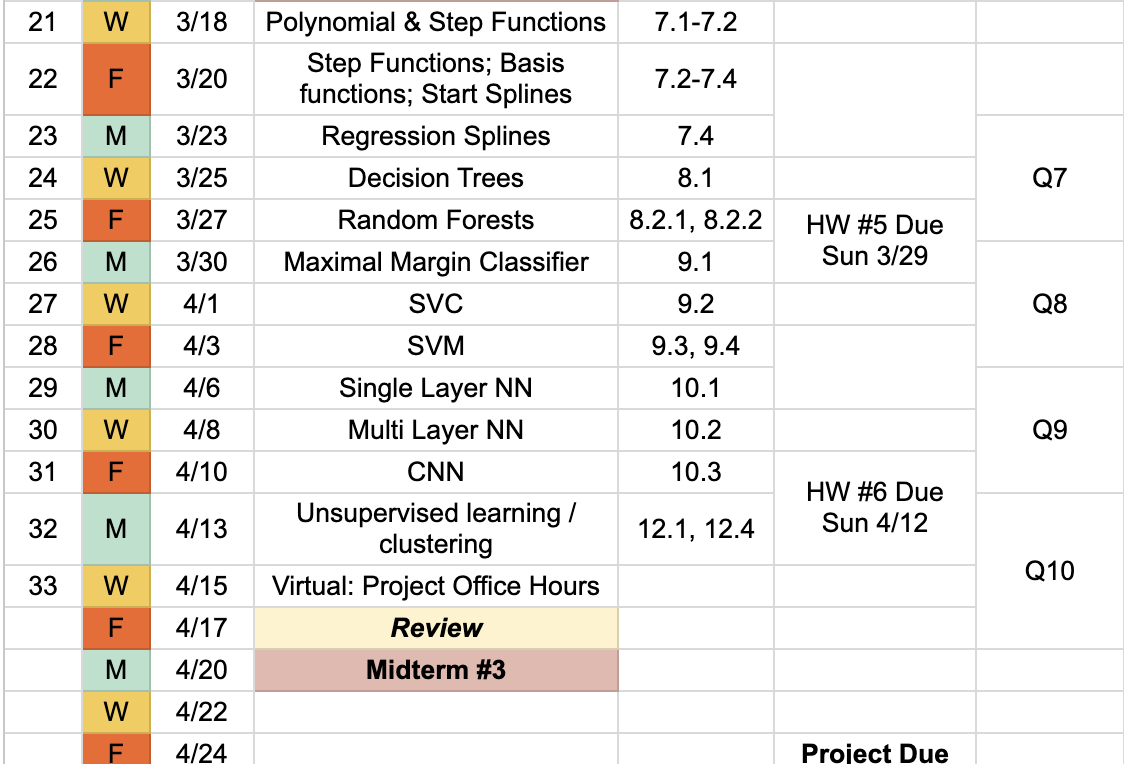
\includegraphics[align = c, width = .8\textwidth]{Schedule-S26-3.png}

\end{columns}

\end{frame}
%--- Next Frame ---%



%==========
\section{Previously}
%==========
\begin{frame}[c]{First decision tree example}

\begin{columns}
\column{.25\textwidth}
\centering
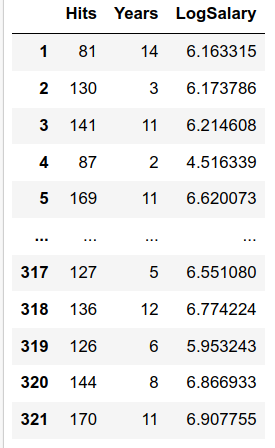
\includegraphics[width = \textwidth, align = c]{Hitters-TreeSlides-OnlyLog.png}
\column{.35\textwidth}
\footnotesize
\InstructorList{
  \item Top split assigns observations with Years$<4.5 $to left branch
	\item Return mean response for players with that.
	\item Predictions:
	\InstructorList{
	  \item  mean log salary is 5.107, so returns $\exp(5.107) = \$165.174 $ thousand dollars
		\item $5.999 \Rightarrow \$402,834$
		\item $6.740 \Rightarrow \$845,346$
	}
}

\column{.35\textwidth}
\centering
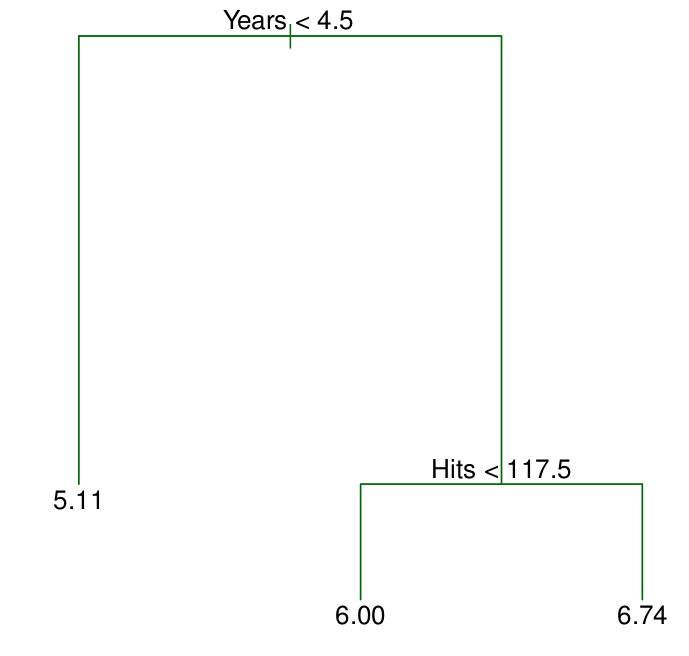
\includegraphics[width = \textwidth, align = c]{Fig8-1}
\end{columns}

\end{frame}
%--- Next Frame ---%


\begin{frame}[c]{Viewing Regions Defined by Tree}

\begin{columns}
\column{.35\textwidth}
\centering
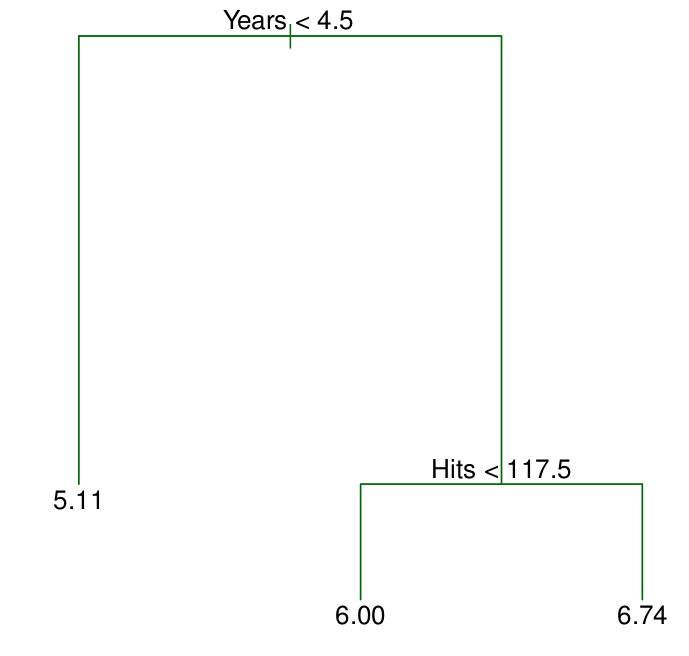
\includegraphics[width = \textwidth, align = c]{Fig8-1}
\column{.45\textwidth}
\centering

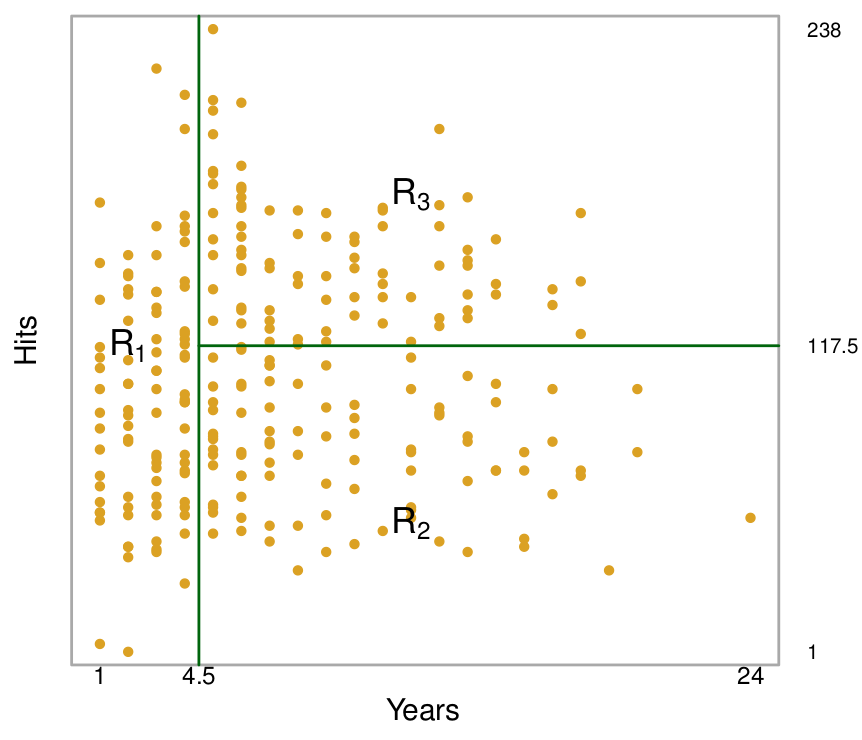
\includegraphics[width = \textwidth, align = c]{Fig8-2}
\end{columns}

\end{frame}
%--- Next Frame ---%


\begin{frame}[c]{How do we actually get the tree? Two steps}

\begin{columns}
\column{.45\textwidth}
\centering
\begin{enumerate}
	\item We divide the predictor space -- that is, the set of possible values for $X_1 , X_2 , \cdots , X _p$ --- into $J$ distinct and non-overlapping regions, $R_1 , R_2 , \cdots, R_J $.
	\item For every observation that falls into the region $R_j$, we make the same prediction $=$ the mean of the response values for the training observations in $R_j $.
\end{enumerate}
\column{.45\textwidth}
\centering
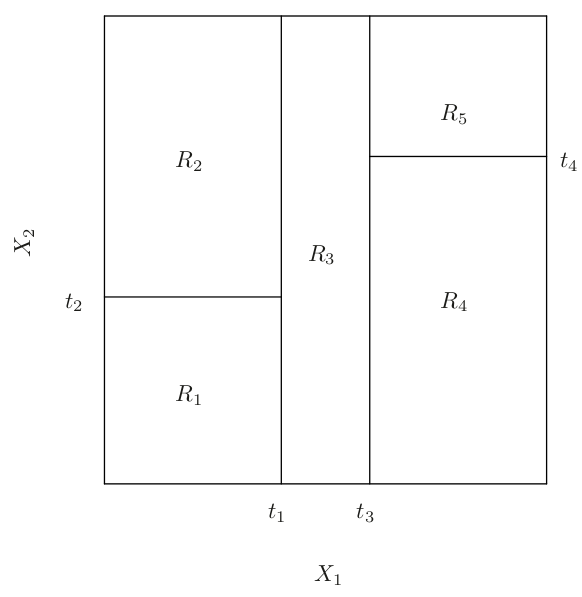
\includegraphics[width = \textwidth, align = c]{Fig8-3b}
\end{columns}

\end{frame}
%--- Next Frame ---%



\begin{frame}[c]{Recursive binary splitting}

\begin{columns}
\column{.3\textwidth}
\centering
\textbf{Goal:}

Find boxes $R_1,\cdots,R_J$ that minimize

\begin{equation*}
	\sum_{j=1}^J \sum_{i \in R_j} (y_i-\hat y_{R_j})^2
\end{equation*}
$\hat y_{R_j} = $ mean response for training observations in $j$th box

\column{.45\textwidth}

Pick $s$ so that splitting into $\{X \mid X_j < s\}$ and $\{X \mid X_j \geq s\}$ results in largest possible reduction in RSS:
\begin{align*}
	R_1(j,s) = \{X \mid X_j < s\}\\
	R_2(j,s) = \{X \mid X_j \geq s\}\\
\end{align*}
\begin{equation*}
	\sum_{i \mid x_i \in R_1(j,s)}(y_i - \hat y _{R_1})^2
	+
	\sum_{i \mid x_i \in R_2(j,s)}(y_i - \hat y _{R_2})^2
\end{equation*}

\column{.2\textwidth}
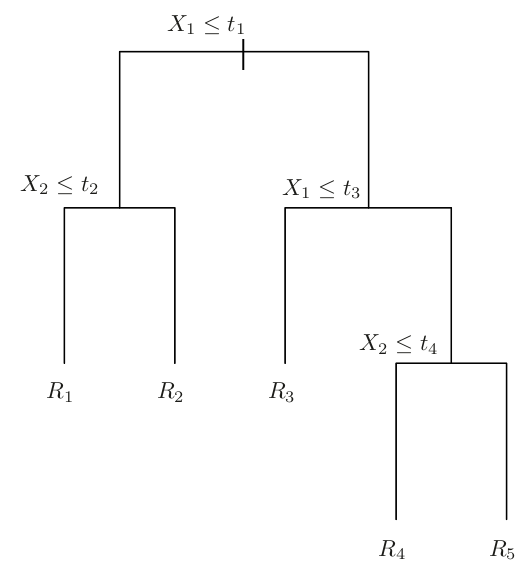
\includegraphics[width = \textwidth, align = c]{Fig8-3c}
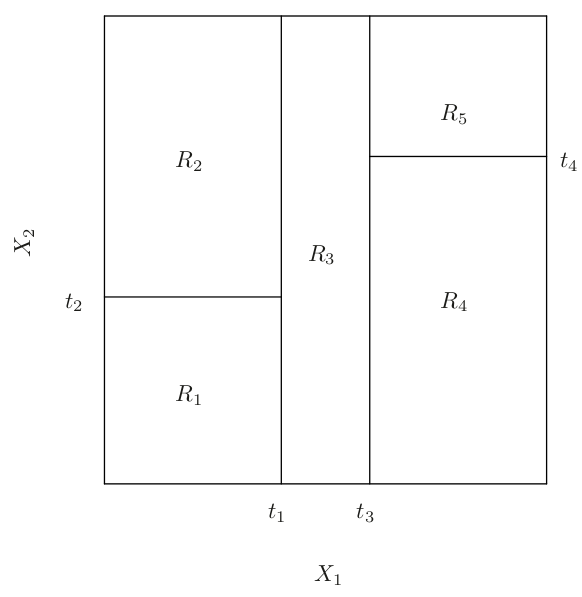
\includegraphics[width = \textwidth, align = c]{Fig8-3b}
\end{columns}

\end{frame}
%--- Next Frame ---%


\begin{frame}[c]{Pruning}

\begin{columns}
\column{.3\textwidth}
\centering
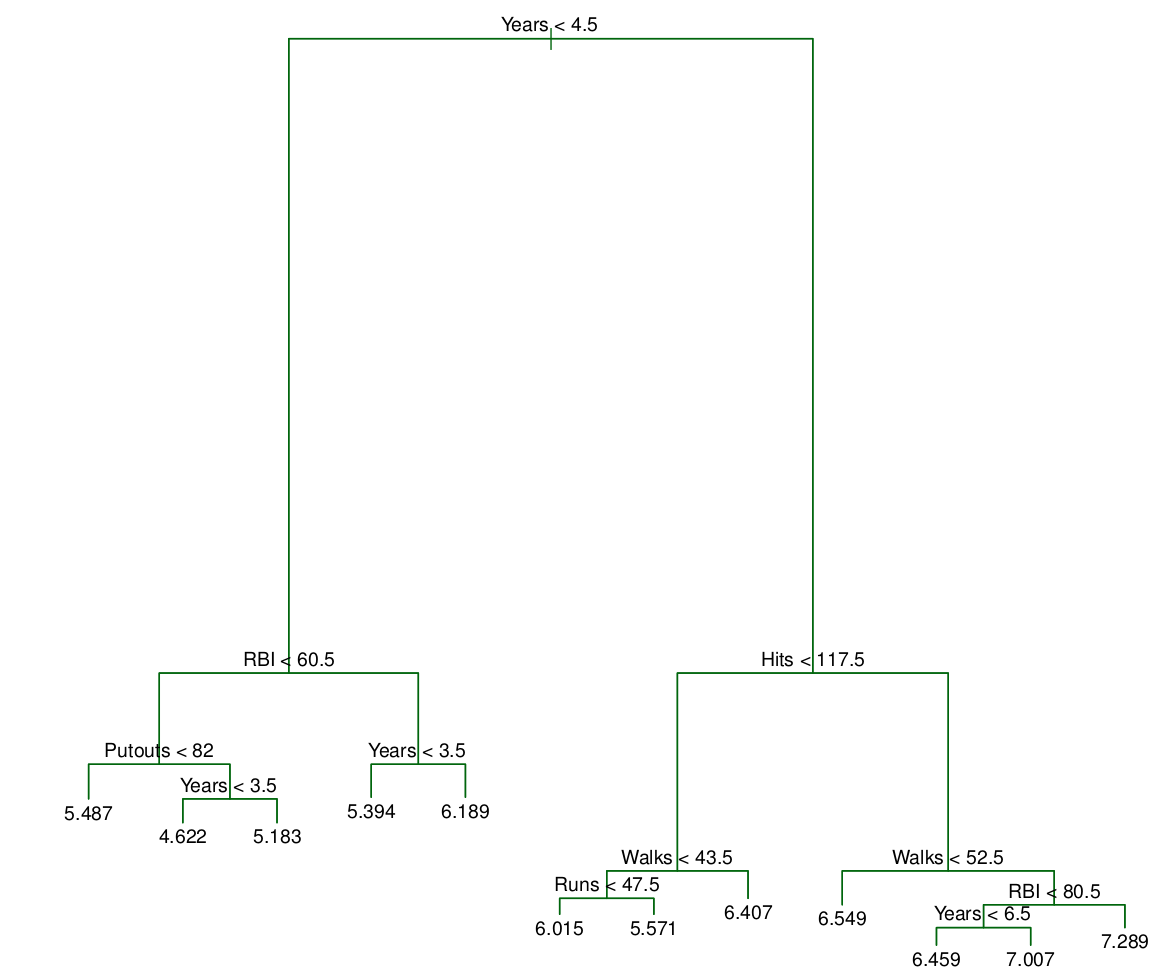
\includegraphics[width = \textwidth, align = c]{Fig8-4}
\column{.3\textwidth}
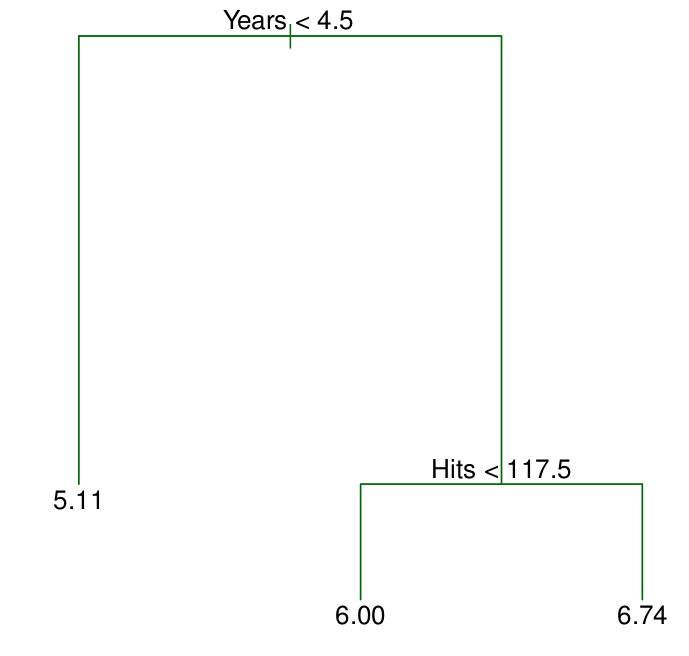
\includegraphics[width = \textwidth, align = c]{Fig8-1}
\column{.35\textwidth}
\centering
\InstructorList{
  \item Big trees leave you open to potential overfitting
  \item One option is maximum deapth 
  \item Another is Weakest link pruning 
	% \item Could just stop building earlier, but that's short sighted
	% \item Instead, grow a big tree and prune it back
	% \item Find subtree with best test error rate
	% \item Too many subtrees to test them all
}


\end{columns}

\end{frame}
%--- Next Frame ---%

% \begin{frame}[c]{Weakest Link Pruning }
% 	{Also called Cost complexity pruning}

% \begin{columns}
% \column{.45\textwidth}
% \centering

% For every $\alpha$, there is a subtree $T$ that minimizes:
% \begin{equation*}
% 	\sum_{m=1}^{|T|} \sum_{i \mid x_i \in R_m } (y_i - \hat y_{R_m})^2 + \alpha |T|
% \end{equation*}

% \begin{itemize}
% 	\item $|T| = $ number of terminal nodes of $T$
% 	\item $R_m$ is rectangle for $m$th terminal node
% 	\item $\hat y_{R_m}$ is mean of training observations in $R_m$
% \end{itemize}
% \column{.45\textwidth}
% \centering
% \begin{itemize}
%   \item $\alpha=0$ gets entire tree
% 	\item Increasing $\alpha$ penalizes size of tree
% 	\item Branches pruned from tree in nested and predictable fashion
% 	\item Easy to get trees for all vales of $\alpha$
% 	\item Pick $\alpha $ via CV
% \end{itemize}

% 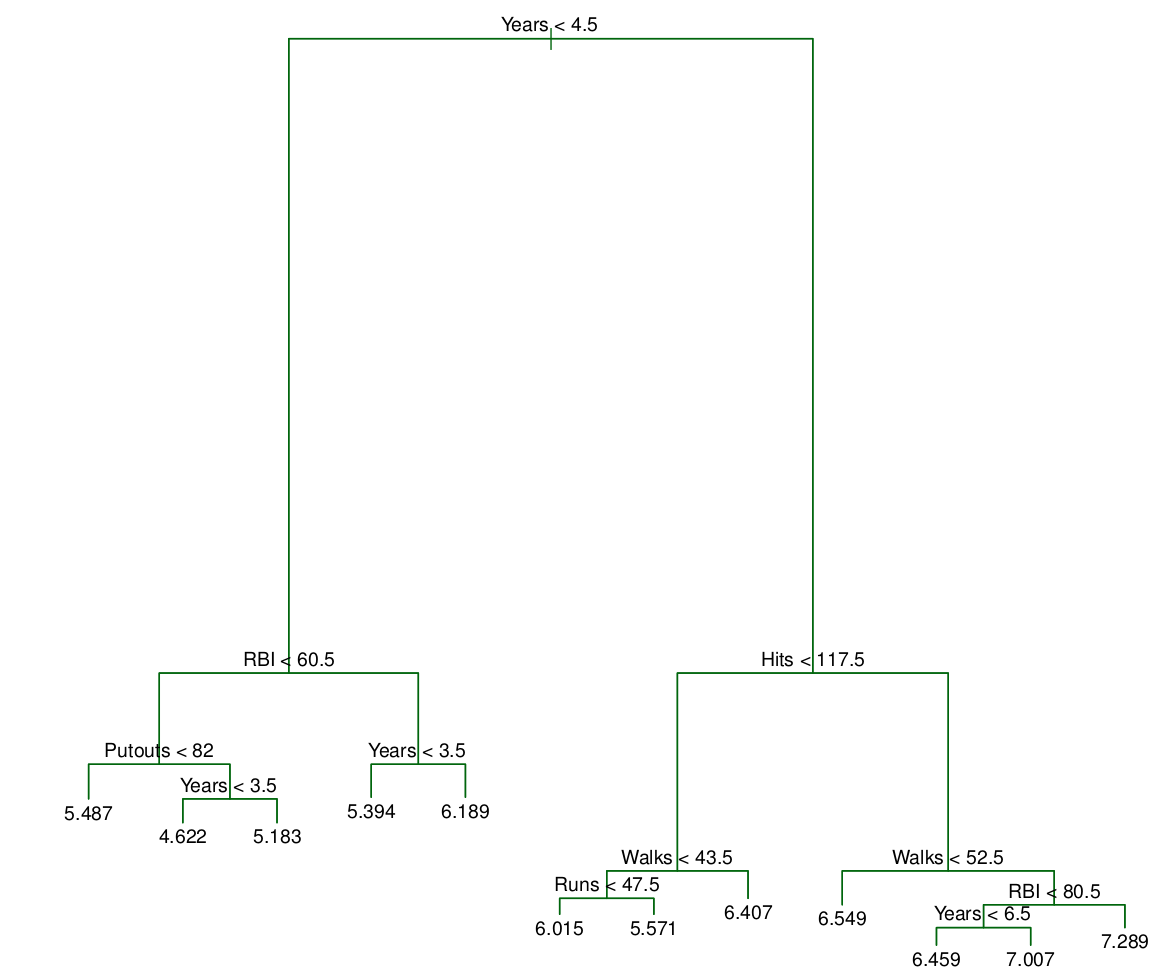
\includegraphics[width = .49\textwidth, align = c]{Fig8-4}
% 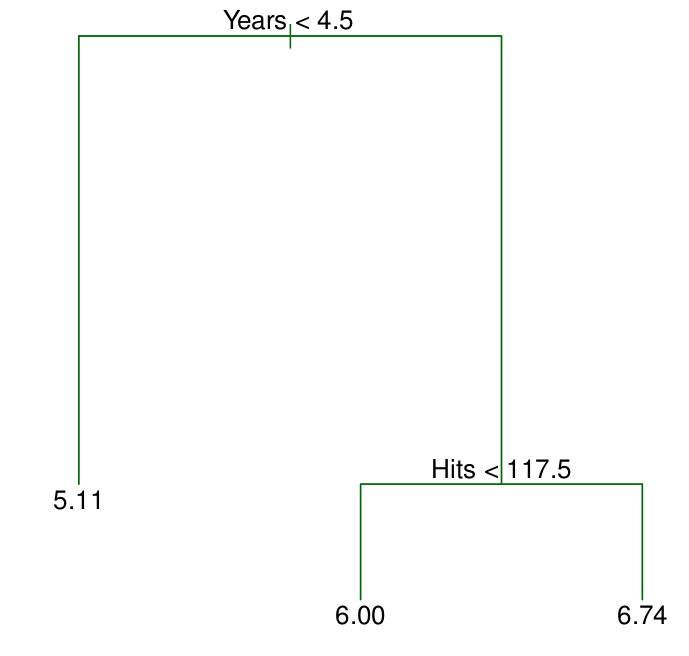
\includegraphics[width = .49\textwidth, align = c]{Fig8-1}
% \end{columns}

% \end{frame}
%--- Next Frame ---%
% \begin{frame}[c]{Algorithm version}

% \begin{columns}
% \column{.65\textwidth}
% \centering
% 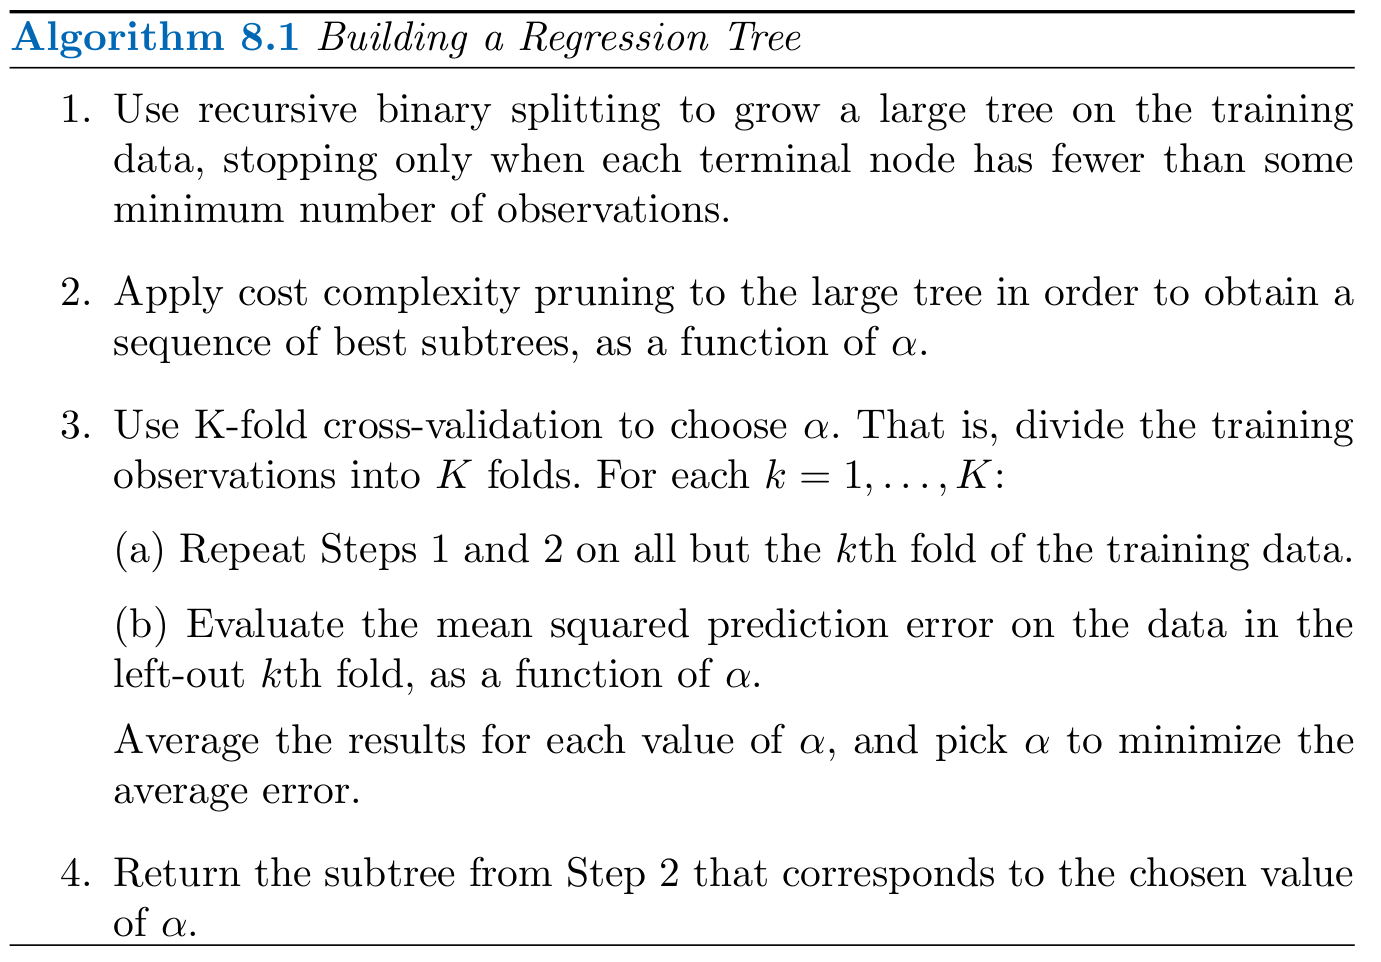
\includegraphics[width = \textwidth, align = c]{Alg8-1}

% \end{columns}

% \end{frame}
%--- Next Frame ---%
\begin{frame}[t]{Classification version}

\begin{columns}
\column{.45\textwidth}
\centering

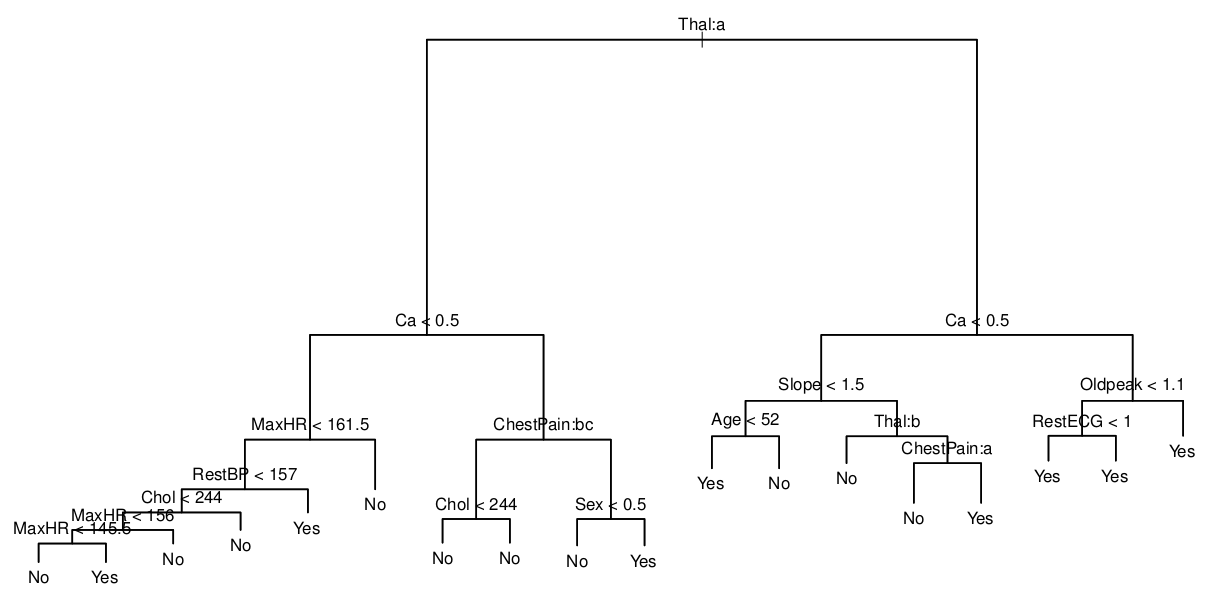
\includegraphics[width = \textwidth, align = c]{Fig8-6a}

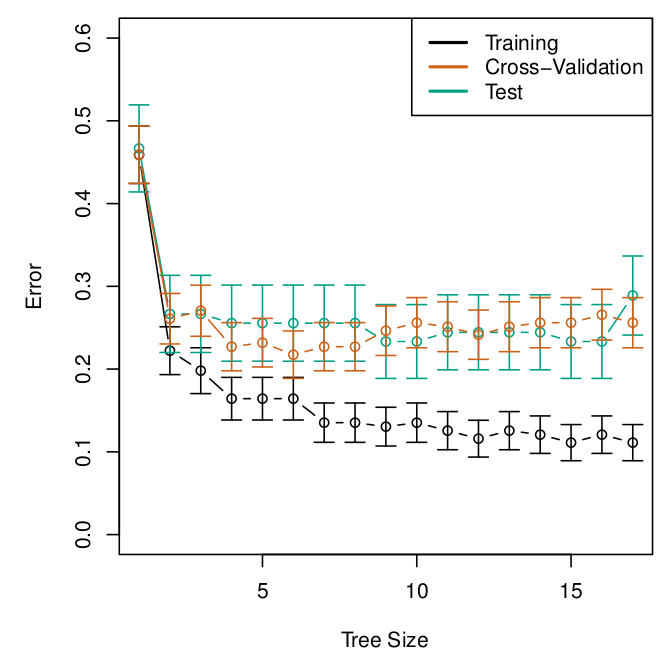
\includegraphics[width = .49\textwidth, align = c]{Fig8-6b}
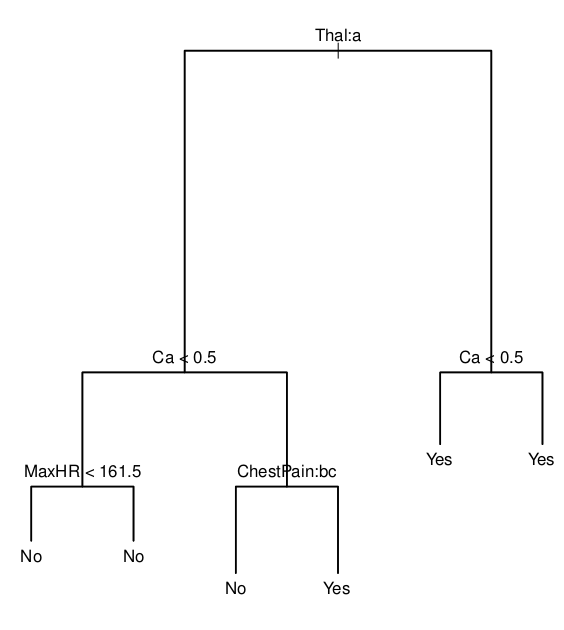
\includegraphics[width = .49\textwidth, align = c]{Fig8-6c}
\column{.45\textwidth}
\centering
\textbf{Evaluating the splits:}
\begin{itemize}
	\item $\hat p_{mk} = $ proportion of training observations in $R_m$ from the $k$th class
	\item Error: $E = 1-\max_{k}(\hat p_{mk})$
	\item Gini index:
	\begin{equation*}
		G = \sum_{k=1}^K \hat p_{mk} (1-\hat p_{mk})
	\end{equation*}
	% \item Entropy:
	% \begin{equation*}
	% 	D = - \sum_{k=1}^K \hat p_{mk} \log \hat p _{mk}
	% \end{equation*}
\end{itemize}

\end{columns}

\end{frame}
%--- Next Frame ---%
\begin{frame}[c]{Linear models vs trees }
	\InstructorList{
	  \item Trying to predict green vs yellow
	}
	

\begin{columns}
\column{.45\textwidth}
\centering
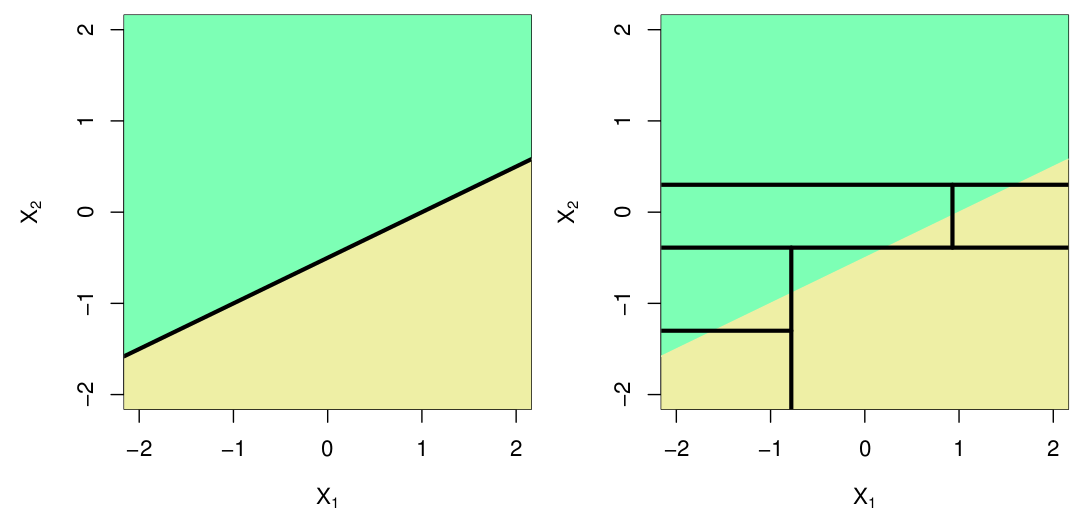
\includegraphics[width = \textwidth, align = c]{Fig8-7-top}
\InstructorNotes{Obviously linear does better here}
\column{.45\textwidth}
\centering
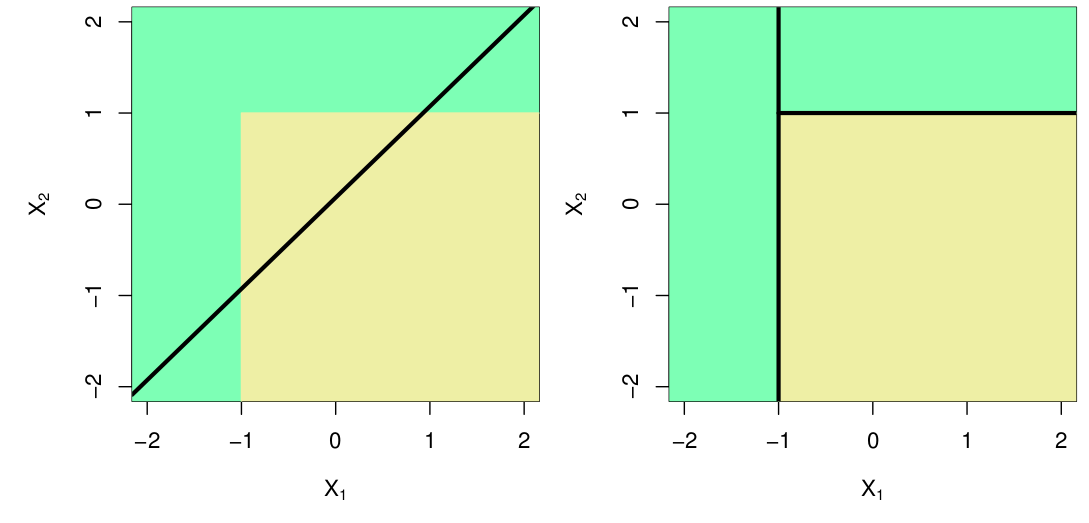
\includegraphics[width = \textwidth, align = c]{Fig8-7-bottom}
\InstructorNotes{Not going to beat this case though}
\end{columns}

\end{frame}


% --- Next Frame ---%
\begin{frame}[t]{What will your learn today?}
	\begin{itemize}
		\item What does bagging of decision trees accomplish?
		\item How do you use out of bag error estimation for decision trees?
			\begin{itemize}
				\item You should be able to describe this for both regression and classification trees.
			\end{itemize}
		\item What problem of bagging does using random forest address?
		\item What is the relationship between random forest and bagging?
	\end{itemize}

\end{frame}


%=====
\section{8.2.1 Bagging}
%=====

\begin{frame}[t]{Use ensemble of trees to reduce variance}

\begin{columns}
\column{.45\textwidth}
% \centering
% Averaging a set of observations reduces variance:
% \begin{itemize}
% 	\item $n$ independent observations $Z_1,\cdots, Z_n$ each with variance $\sigma^2$
% 	\item Variance of the mean $\bar Z$ is $\sigma^2/n$
% \end{itemize}

\textbf{Want to do (but can't):} \\
Build separate models from independent training sets, and average resulting predictions:
\begin{itemize}
	\item $\hat f^1(x), \cdots, \hat f^B(x)$ for $B$ separate training sets
	\item Return the average
	\begin{equation*}
		\hat f_{avg}(x) = \frac{1}{B} \sum_{b=1}^B \hat f^b(x)
	\end{equation*}

\end{itemize}
\InstructorList{
  \item Decreases variance, but not practical
}

\column{.45\textwidth}
% \centering

\textbf{Boostrap modification:}
\begin{itemize}
	\item Work with fixed data set
	\item Take $B$ samples from this data set (with replacement)
	\item Train method on $b$th sample to get $\hat f^{*b}(x)$
	\item Return average of predictions (regression)
	\begin{equation*}
		\hat f_{bag}(x) = \frac{1}{B} \sum_{b=1}^B \hat f^{*b}(x)
	\end{equation*}
	or majority vote (classification)
\end{itemize}



\end{columns}

\end{frame}
%--- Next Frame ---%

\begin{frame}[t]{Tree version}
	\centering
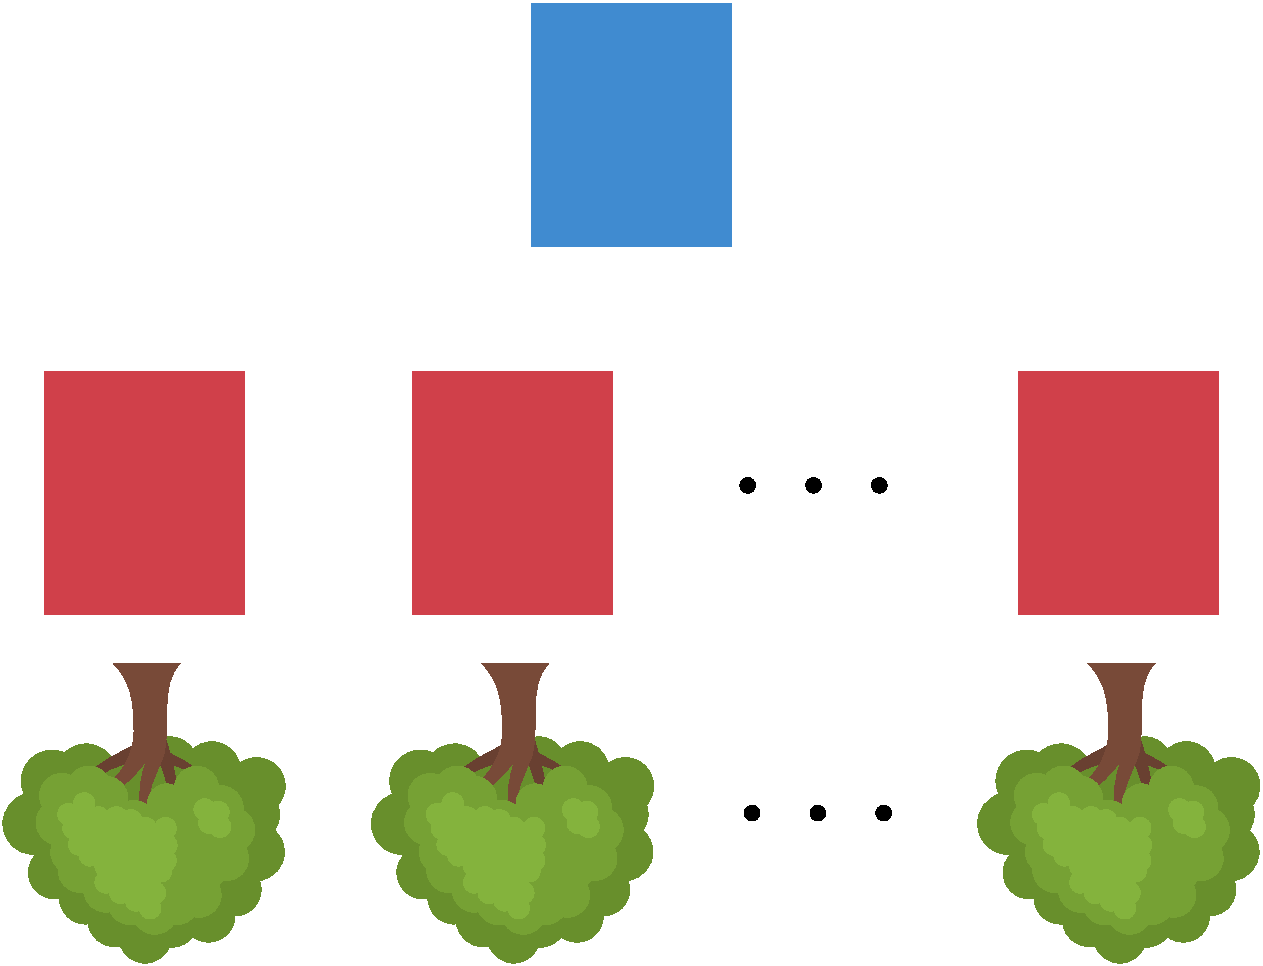
\includegraphics[width = .6\textwidth, align = c]{TreeBaggingCartoon}
\InstructorNotes{
	\begin{minipage}
		{.35\textwidth}
		\InstructorList{
		\item Blue is original data set $X:n \times p$ 
		\item Red are the subsampled  data sets 
		\item Build a tree from each 
		\item Get prediction from each, return the average
		}
	\end{minipage}
}
\end{frame}
%--- Next Frame ---%
\begin{frame}[c]{Prediction on new data point }
\InstructorNotes{New data point goes in, run through each tree, average outputs}
\centering
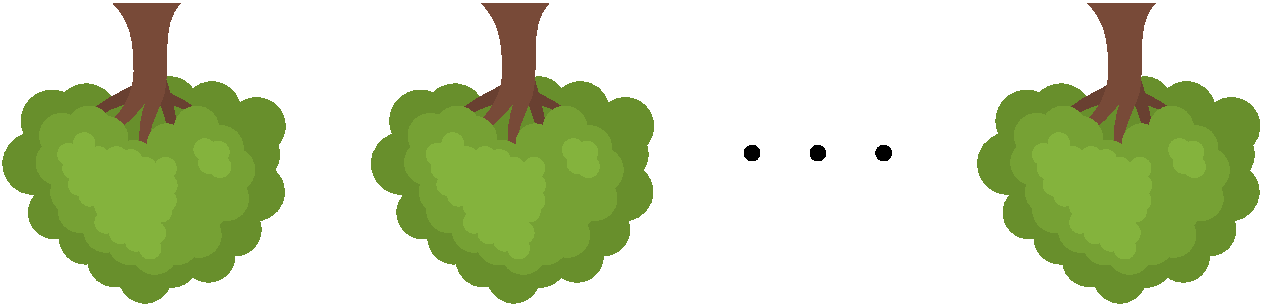
\includegraphics[width = .6\textwidth]{TreeBaggingCartoon-OnlyTrees}

\end{frame}
%--- Next Frame ---%

% \begin{frame}[t]{Bagging vs Bootstrap}

% \begin{columns}
% \column{.45\textwidth}
% \centering
% \textbf{Bootstrap}

% \InstructorList{
%   \item Getting subset of data by subsampling
% 	\item Better name: Bootstrap sample
% }

% \column{.45\textwidth}
% \centering

% \textbf{Bagging}

% \InstructorList{
%   \item Taking the predicted values and averaging them
% 	\item Better name: Bootstrap aggregation
% 	\item Note: bagging can be done on many different kinds of models. We just happen to be doing it here on trees
% }
% \end{columns}

% \end{frame}
%--- Next Frame ---%
\begin{frame}[t]{Example: Heart classification data}

\begin{columns}
\column{.45\textwidth}
\centering
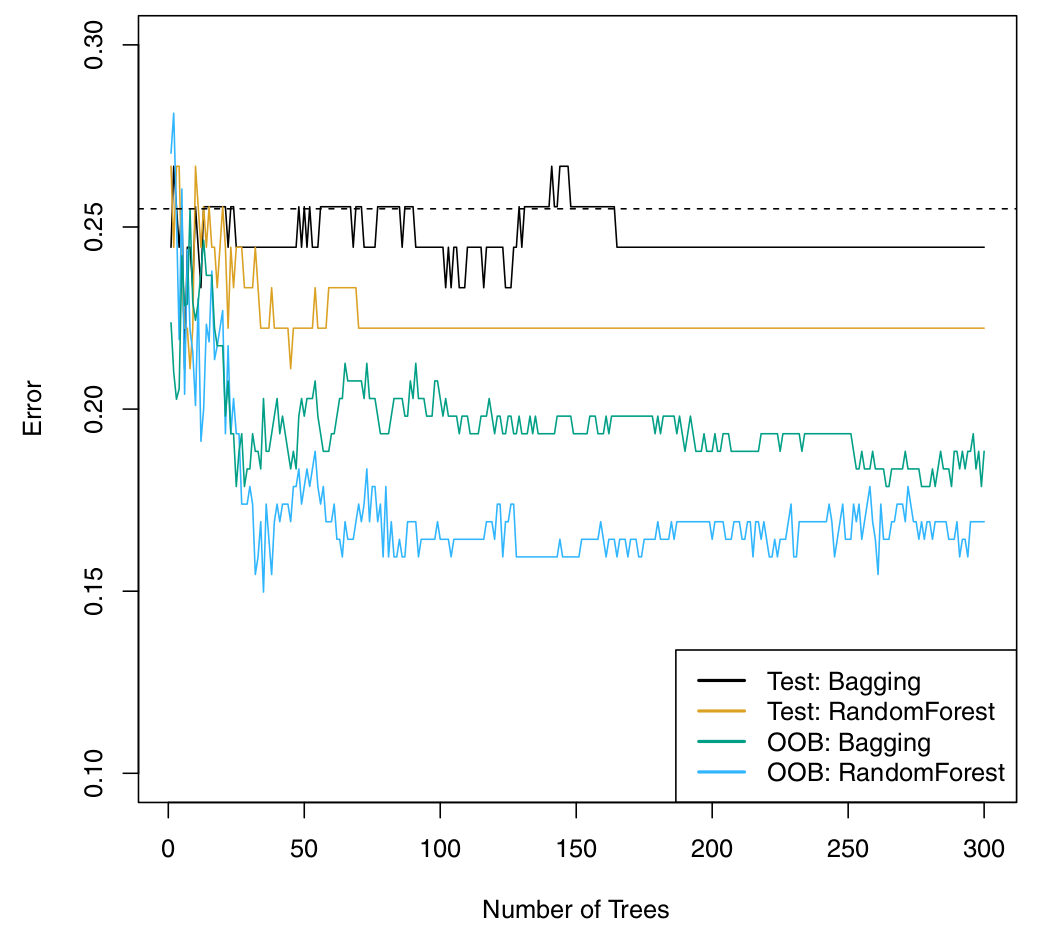
\includegraphics[width = \textwidth]{Fig8-8}
\column{.45\textwidth}
\centering

\InstructorList{
\item Example is done for classification
  \item Ignore everything but black lines
	\item Dashed is test error from single classification tree
	\item Solid black is from bagged version
	\item Note that you just need $B$ big enough for error to stabilize, so about 100 is good
	\item emphasize that number of trees is not a flexibility parameter
}

\end{columns}

\end{frame}
%--- Next Frame ---%
\begin{frame}[t]{Out of Bag Error Estimation}

\begin{columns}
\column{.45\textwidth}
\centering
\begin{itemize}
	\item On average, bootstrap sample uses about 2/3 of the data \InstructorNotes{We did this homework problem a while ago I think? Ch 5, Ex. 2}
	\item Remaining observations not used are called \textit{out-of-bag} (OOB) observations
	\item For each observation, run through all the trees where it wasn't used for building
	\item Return the average (or majority vote) of those as test prediction! rather law of large number
	\item Bootstraped version of LOOCV.
\end{itemize}
\column{.45\textwidth}
\centering
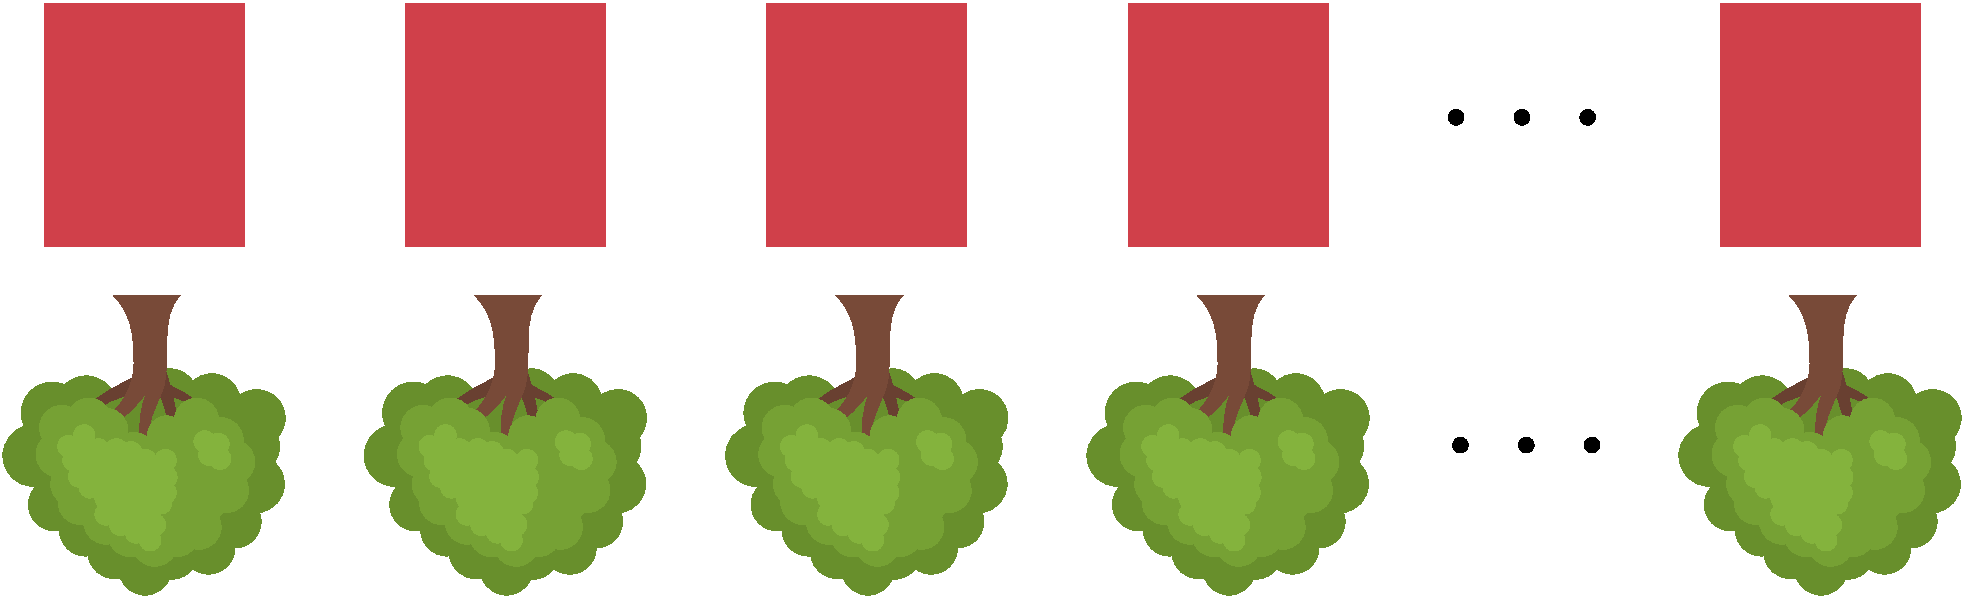
\includegraphics[width = \textwidth]{TreeBaggingCartoon-MoreTrees}
\end{columns}

\end{frame}
%--- Next Frame ---%

\begin{frame}[t]{Error using OOB}

\begin{columns}
\column{.45\textwidth}
\centering
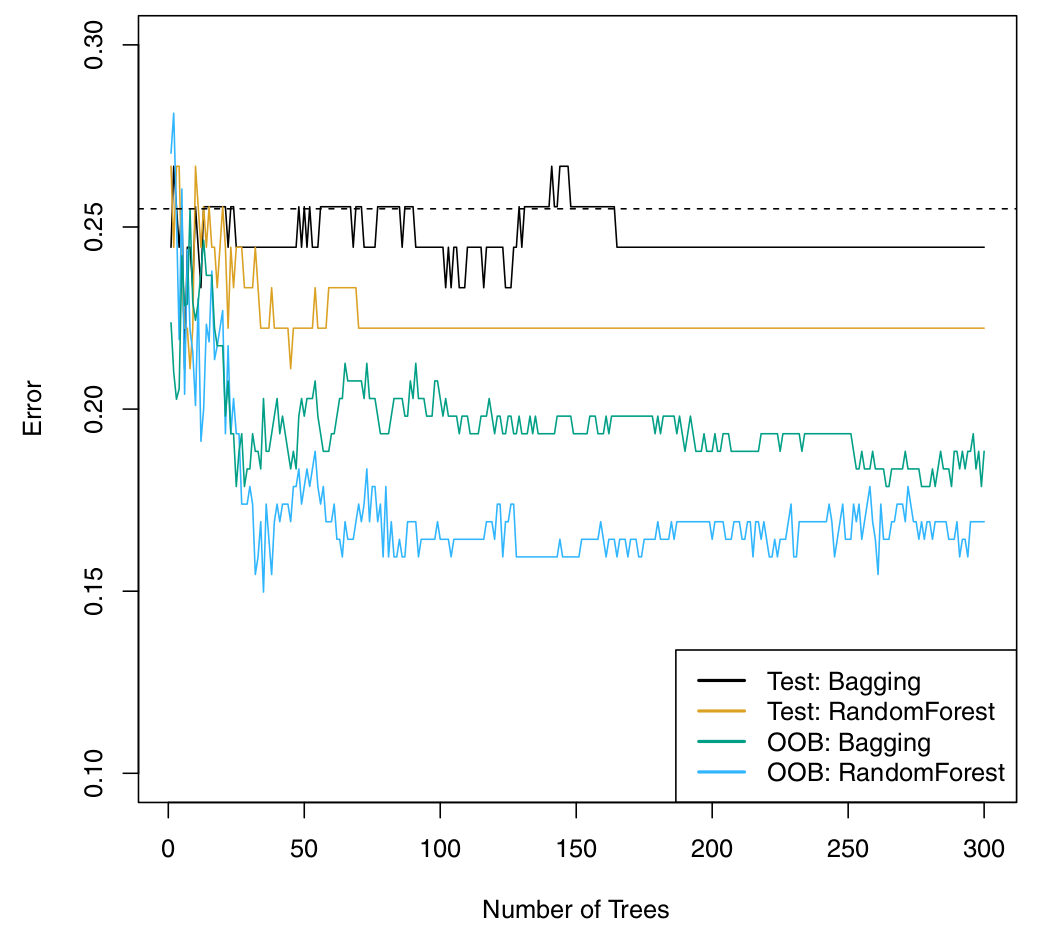
\includegraphics[width = \textwidth]{Fig8-8}
\column{.45\textwidth}
\centering

\InstructorList{
  \item Green line has OOB error
  \item note OOB is averaged B/3 predictions per observation 
	\item Book says the fact that the OOB value is so much lower is just random chance?
}

Test your understanding: \href{https://PollEv.com/multiple_choice_polls/Ml8a7cfP8JC1EUABn4cSU/respond}{PollEv}

\end{columns}

\end{frame}
%--- Next Frame ---%

% {
% \setbeamercolor{background canvas}{bg=Apricot!25}
% \begin{frame}[t]{Bagging code example}
% \begin{columns}
% \column{.45\textwidth}
% \centering
% \column{.45\textwidth}
% \centering
% \end{columns}
% \end{frame}
% }
%--- Next Frame ---%

%=====
\section{Random Forests}
%=====



\begin{frame}[t]{The idea }

\begin{columns}
\column{.45\textwidth}
\centering
\begin{itemize}
	\item Goal is to decorrelate the bagged trees:
	\begin{itemize}
		\item If there is a strong predictor, the first split of most trees will be the same
		\item Most or all trees will be highly correlated
		\item Averaging highly correlated quantities doesn't decrease variance as much as uncorrelated
	\end{itemize}
\end{itemize}
\column{.45\textwidth}
\centering
\begin{itemize}
	\item The random forest fix:
	\begin{itemize}
		\item Each time a split is considered, only use a random subset of $m$ the predictors
		\item Fresh sample taken every time
		\item Typically $m \approx \sqrt p$
		\item On average, $(p-m)/p$ of splits won't consider strong predictor
		\item $m = p$ gives back bagging
	\end{itemize}
\end{itemize}
\end{columns}

\end{frame}
%--- Next Frame ---%



\begin{frame}[t]{Example on gene expression}

\begin{columns}
\column{.45\textwidth}
\centering
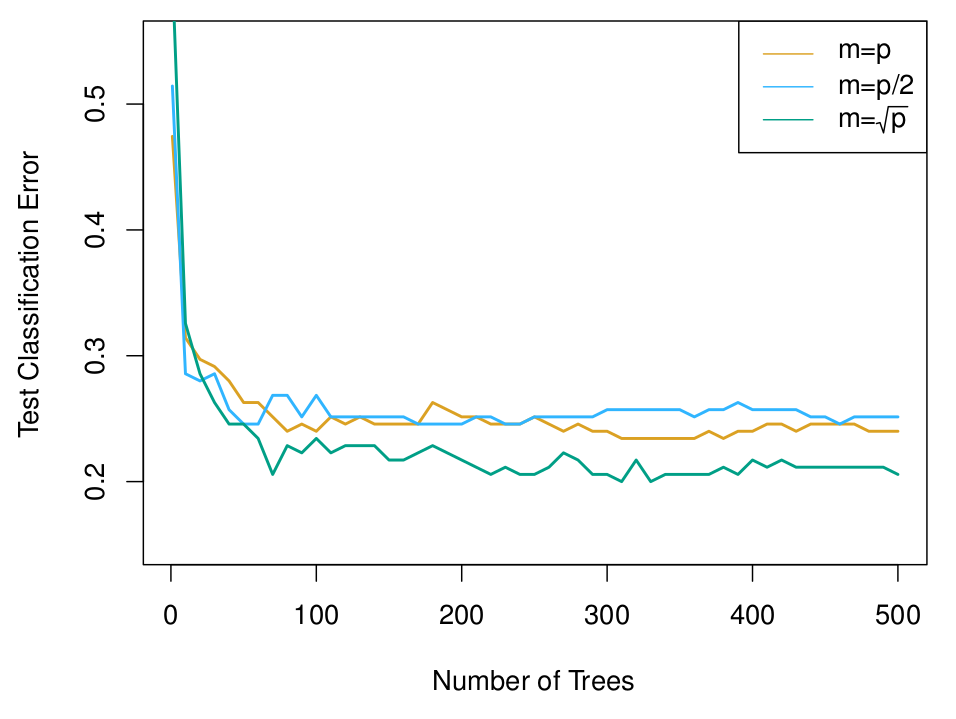
\includegraphics[width = \textwidth]{Fig8-10}
\column{.45\textwidth}
\centering
\footnotesize
\InstructorList{
	\item Helpful for large $p$
	\item Predict one of 14 types of cancer (15 total levels), use 500 genes with most variance
	\item Random split to train and test set, three values of $m$
	\item Error rate of single tree: 45.7\%
	\item Null rate 75.4\% (classify each into the dominant overall class, here the healthy class)
	\item 400 trees enough for good performance
	\item $m=\sqrt p$ small improvement over bagging $(m=p)$ in this case

}

\end{columns}


\end{frame}
%--- Next Frame ---%
{
\setbeamercolor{background canvas}{bg=Apricot!25}
\begin{frame}[t]{Coding time!}
\begin{columns}
\column{.45\textwidth}
\centering
\column{.45\textwidth}
\centering
\end{columns}
\end{frame}
}
%--- Next Frame ---%

% %==========
% \section{Boosting}
% %==========

% \begin{frame}[t]{Boosting idea}

% \begin{columns}
% \column{.45\textwidth}
% \centering
% 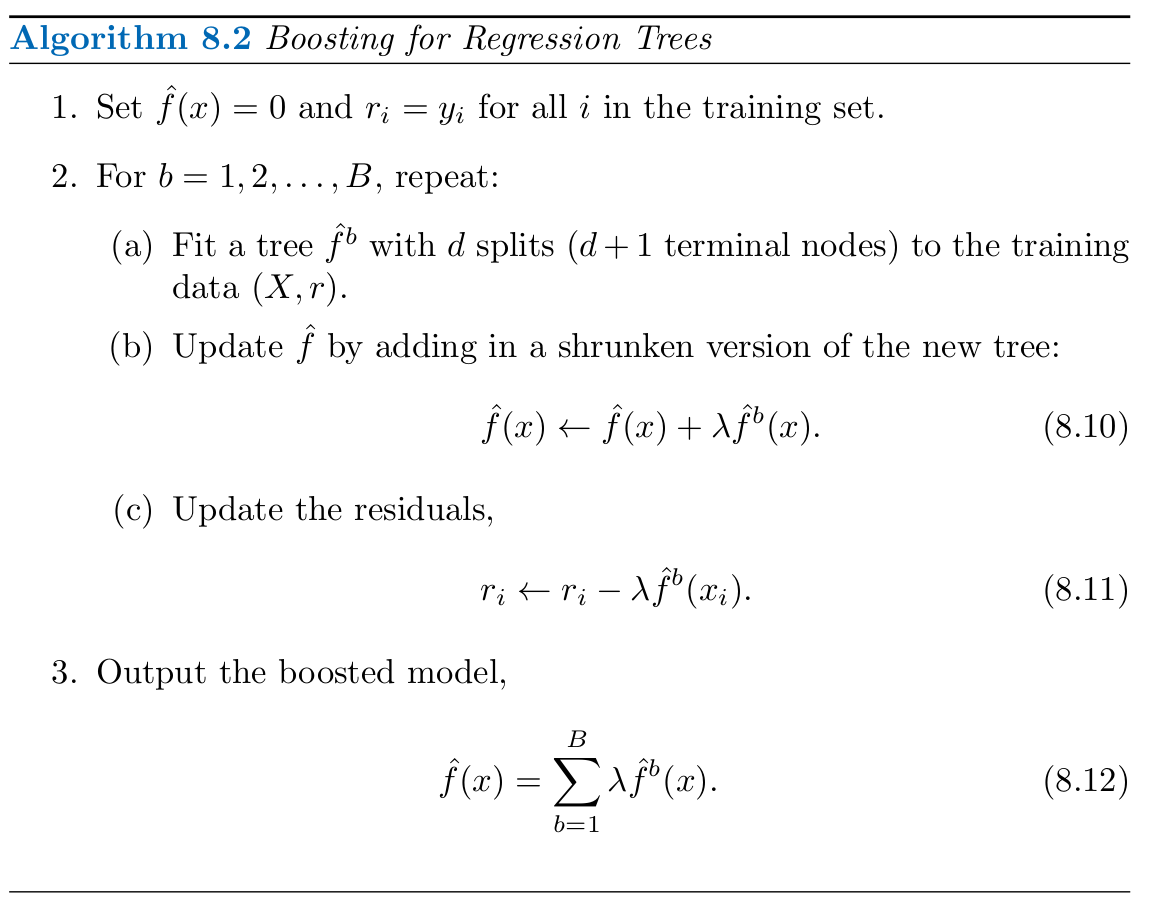
\includegraphics[width = \textwidth, align = c]{Alg8-2}
% \column{.45\textwidth}
% \centering
% \InstructorList{
%   \item creates group of trees
% 	\item does this by building on modified data rather than bootstrap sample
% 	\item Trees are grown sequentially
% 	\item Learns slowly..... shrinkage parameter slows down the process
% 	\item parameters: $B$, $\lambda$, $d = depth$
% }

% \end{columns}

% \end{frame}
% %--- Next Frame ---%

% \begin{frame}[t]{Example }

% \begin{columns}
% \column{.45\textwidth}
% \centering



% \column{.45\textwidth}
% \centering
% 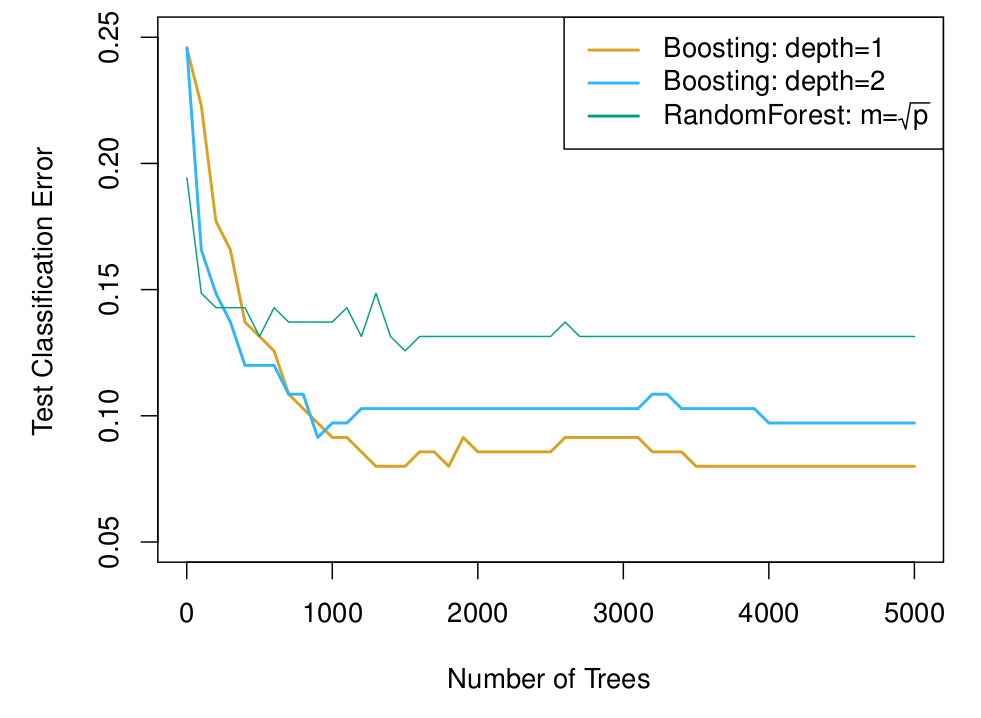
\includegraphics[width = \textwidth, align = c]{Fig8-11}

% \end{columns}

% \end{frame}
% %--- Next Frame ---%

% %==========
% \section{BART}
% %==========



% \begin{frame}[t]{BART}

% \begin{columns}
% \column{.45\textwidth}
% \centering
% \begin{itemize}
% 	\item Create trees in random manner (like bagging, random forests, and boosting)
% 	\item Try to capture signal not yet accounted for (like boosting)
% 	\item Change how trees are generated
% \end{itemize}
% \column{.45\textwidth}
% \centering

% \end{columns}

% \end{frame}
% %--- Next Frame ---%
% \begin{frame}[t]{Notation}

% \begin{columns}
% \column{.45\textwidth}
% \centering
% \begin{itemize}
% 	\item $K$: number of regression trees
% 	\item $B$: number of iterations to run the BART algorithm
% 	\item $\hat f_k^b(x)$: Prediction at $x$ for $k$th regression tree for $b$th iteration
% 	\item $\hat f^b(x) = \sum_{k=1}^K \hat f_k^b$
% \end{itemize}
% \column{.45\textwidth}
% \centering

% \end{columns}

% \end{frame}
% %--- Next Frame ---%

% \begin{frame}[t]{BART Algorithm idea}

% \begin{columns}
% \column{.45\textwidth}
% \centering
% \begin{itemize}
% 	\item Start with single root node for each tree
% 	\begin{equation*}
% 		\hat f_k^1(x) = \frac{1}{nK} \sum_{i=1}^n  y_i
% 	\end{equation*}
% 	\InstructorNotes{Mean of response over number of trees }
% 	\item Update one tree at a time. Update $k$th tree at $b$th iteration, get partial residual:
% 	\begin{equation*}
% 		r_i = y_i - \sum_{k'<k} \hat f_{k'}^b(x_i) - \sum_{k'>k} \hat f_{k'}^{b-1}(x_i)
% 	\end{equation*}
% 	\item Randomly choose pertubation to tree
% \end{itemize}
% \column{.45\textwidth}
% \centering
% 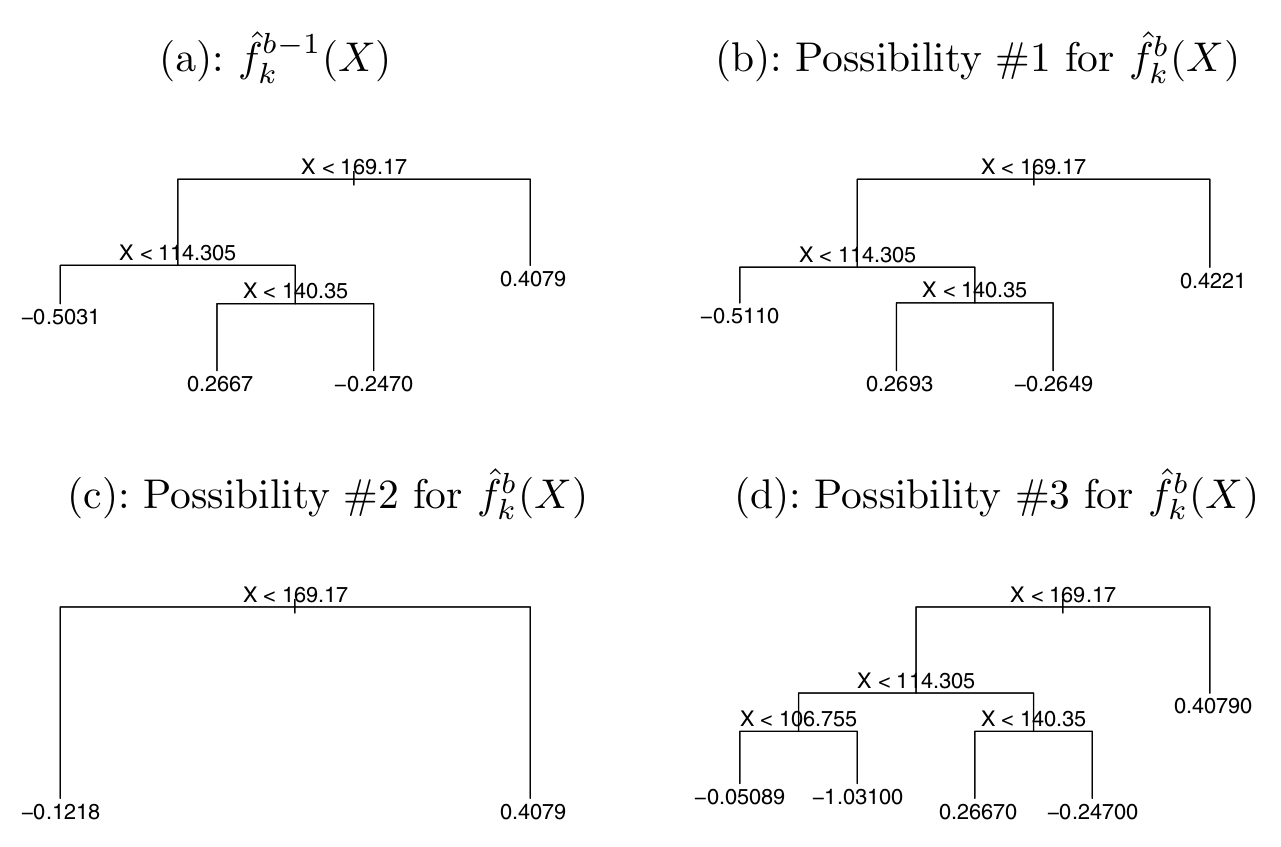
\includegraphics[width = \textwidth, align = c]{Fig8-12}
% \end{columns}

% \end{frame}
% %--- Next Frame ---%
% \begin{frame}[t]{Example}

% \begin{columns}
% \column{.45\textwidth}
% \centering
% 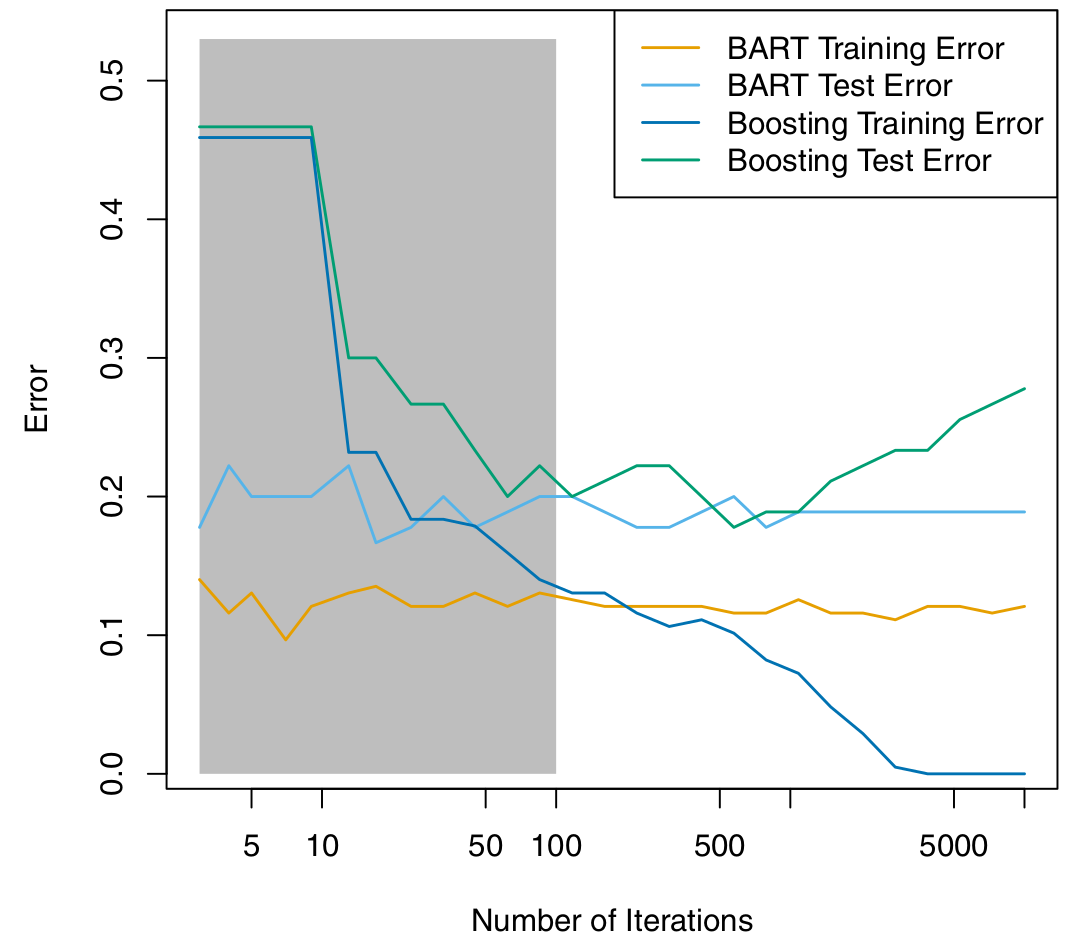
\includegraphics[width = \textwidth, align = c]{Fig8-13}
% \column{.45\textwidth}
% \centering
% \InstructorList{
%   \item Initial burn in period, after that the error rates settle down
% 	\item Small diff between training/test, largely avoids overfitting
% 	\item Markove chain Monte carlo method
% 	\item BART tends to perform well with minimal training
% }

% \end{columns}

% \end{frame}
% %--- Next Frame ---%

%================================================
\begin{frame}[c]{TL:DR}

\begin{columns}
\column{.45\textwidth}
\centering

\begin{itemize}
  \item Bagging: trees grown independently on random samples. Trees tend to be similar to each other, can result in getting caught in local optima
	\item Random forest: trees independently on samples, but split is done using random subset of features

\end{itemize}

\column{.45\textwidth}
\centering
% \InstructorList{
%   \item Boosting: Grow trees sucessively with slow learn approach
% 	\item BART Grow trees successively, but each tree perturbed to avoid local minma.
% }

\end{columns}
\end{frame}
%--- Next Frame ---%




\begin{frame}[t]{Next time}
\begin{columns}
\column{0.45\textwidth}
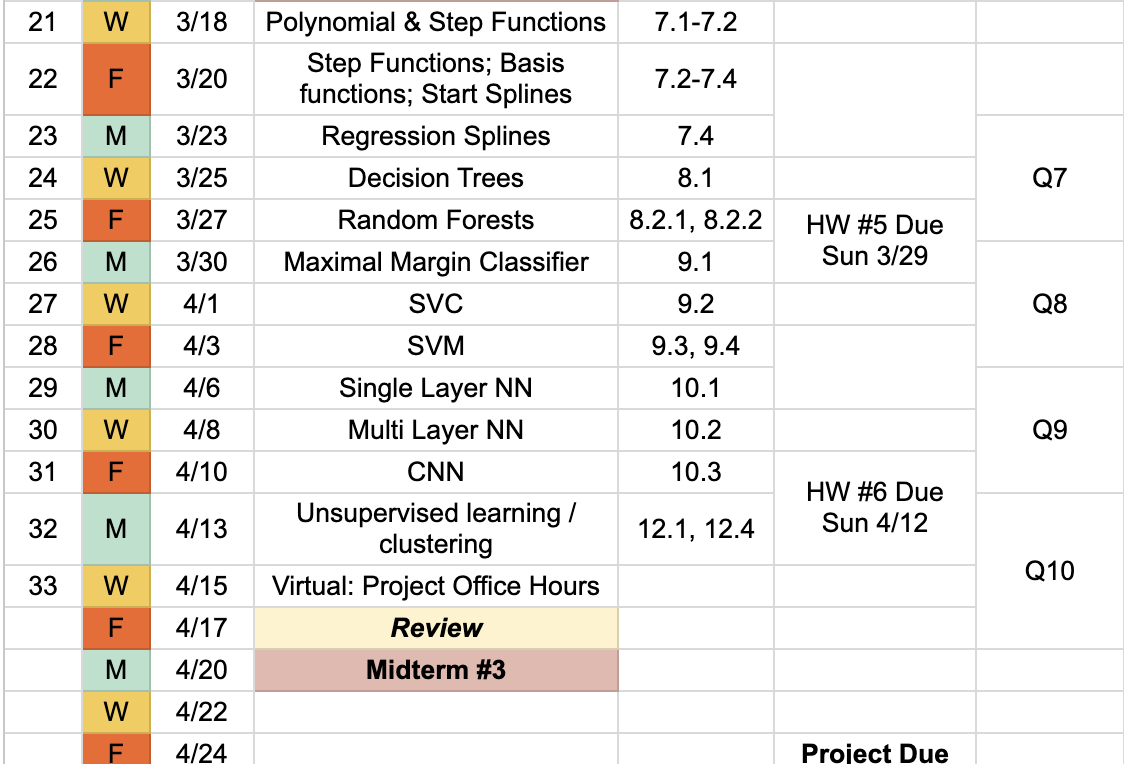
\includegraphics[align = c, width = \textwidth]{Schedule-S26-3.png}

\column{0.45\textwidth}
% Q of the day:

% You have two very different datasets to create two very different models. 

% You have to use random forest on one and bagging on the other. 

% Which one would benefit more from random forest? what criteria would you use for the making the decision? 
% one with few very strong predictors
\end{columns}



\end{frame}
%--- Next Frame ---%


\end{document}
